\documentclass{article}

\usepackage{epcc}
\usepackage[hyphens]{url}
\PassOptionsToPackage{hyphens}{url}
\usepackage[colorlinks=false, hidelinks]{hyperref}
\usepackage{amsmath}
\usepackage[toc,page]{appendix}
\usepackage[table]{xcolor}
\usepackage[marginparsep=30pt]{geometry}
\usepackage{stmaryrd}
\usepackage{algorithm}
\usepackage{algorithmic}
\usepackage{tikz}
\usepackage{pgfplots}
\usepackage{tabu}
\usepackage{longtable}
\usepackage{tabularx}
\usepackage{listings}
\usepackage{fancyref}
\usepackage{relsize}
\usepackage{float}
\usepackage{graphicx}
\usepackage{subcaption}
\usepackage{diagbox}
\usepackage{multirow}
\usepackage{slashbox}
\usepackage{graphics}
\usepackage{booktabs}
\usepackage{natbib}
\usepackage{csquotes}

\usetikzlibrary{%
    arrows,
    arrows.meta,
    decorations,
    backgrounds,
    positioning,
    fit,
    petri,
    shadows,
    datavisualization.formats.functions,
    calc,
    shapes,
    shapes.multipart,
    matrix,
    plotmarks
}

\usepgfplotslibrary{fillbetween, statistics, dateplot}

\pgfplotsset{%
  compat=1.3,
  every non boxed x axis/.style={%
  enlarge x limits=false,
  x axis line style={}%-stealth},
  },
  every boxed x axis/.style={},
  every non boxed y axis/.style={%
  enlarge y limits=false,
  y axis line style={}%-stealth},
  },
  every boxed y axis/.style={},
}

\renewcommand{\labelenumii}{\theenumii}
\renewcommand{\theenumii}{\theenumi.\arabic{enumii}.}

\bibliographystyle{plainnat}
\bibpunct{(}{)}{;}{a}{,}{,}

\begin{document}

\pagenumbering{roman}

\title{Deep Learning on SpiNNaker: Report}
\author{Jonas Fassbender \\ \textit{jonas@fassbender.dev}}
\date{}

\makeEPCCtitle

\newpage

\hspace{0pt}
\vfill

\begin{abstract}
This paper reports on the preliminary research done for the
dissertation project ``Deep Learning on SpiNNaker''
(formerly ``A Tensorflow Backend to SpiNNaker'').
SpiNNaker is a novel neuromorphic, massively parallel and
energy efficient computer architecture designed for the
task of modeling the human brain.
The goal of ``Deep Learning on SpiNNaker'' is to find out,
if SpiNNaker can be used to accelerate the training of
deep neural networks \citep[see e.g.][]{goodfellow2016}.
The preliminary research done for the dissertation phase
in the summer of 2020 is described and all relevant
findings are presented.
Changes made to the initial project proposal are discussed.
An outline in form of a work plan and relevant background
information are presented as well.
A literature review of \citet{nita_2018} is given at the
end of this report.
\end{abstract}

\vfill
\hspace{0pt}

\newpage

\tableofcontents

\newpage

\pagenumbering{arabic}

\section{Introduction} % {{{
\label{sec:intro}

%This paper concerns itself with the dissertation project:
%``Deep Learning on SpiNNaker'', which will be conducted in
%the period from May 2019 to August 2019 as the final work
%of the author to achieve his Master of Science in
%High Performance Computing with Data Science from the
%University of Edinburgh.
%The report is mostly a summary of the preliminary work
%conducted in the months before the actual work on the
%dissertation will be conducted.

SpiNNaker is a digital neuromorphic computer architecture,
designed to model the human brain.
According to the SpiNNaker project's website:
\begin{displayquote}
  SpiNNaker is a novel massively-parallel computer
  architecture, inspired by the fundamental structure and
  function of the human brain, which itself is composed of
  billions of simple computing elements, communicating
  using unreliable spikes \citep{spinn_proj}.
\end{displayquote}
This is rather a gross simplification of what SpiNNaker was
designed for.
Understanding the human brain is one of the biggest
frontiers of science and there are many ideas on how one
can model a complex and still mostly unknown structure such
as the human brain.
Therefore, there are many different proposed neuromorphic
computer architectures and ideas on how to model the human
brain, from early analogue approaches for vision systems
like presented in \citet{mead1989} to large scale digital
architectures like Blue Brain \citep{markram2006}; all
aiming to implement different types of neurons and models
of the human brain efficiently \citep{furber_et_al_2007}.

SpiNNaker is an architecture for the large scale and
real-time modeling of spiking neural networks
\citep{furber_et_al_2006, furber_et_al_2006b,
  furber_et_al_2007}.
\citet{maass1997} describes spiking neural networks as the
third generation of neural networks.
Unlike the second generation neural networks---which we
will deal with in the dissertation project here reported on
in the form of deep learning neural networks---spiking
neural networks incorporate a concept of time in their
action potentials (spikes).
Neural networks of the second generation do not have a
concept of time and fire every time they are activated.
Spiking neural networks are derived from evidence
collected from biological neural systems, which use the timing of
spikes to encode information; they are therefore more closely
representing neural systems of biological life than deep learning
neural networks \citep{maass1997}.

The SpiNNaker chip is a multiprocessor chip, which has 18 ARM
cores, with a Network-on-Chip system for
communication between cores \citep{furber_et_al_2007,
  spinn_proj}.
Each core can model up to 1000 spiking neurons.
The spiking neurons in the neural network communicate with
spike events \citep{furber_et_al_2007}.
Spike events are---like their biological
counterpart---inherently unstable and small.
This is represented in the interconnection hardware.
Small packets (40 or 72 bits) can be send, without
guarantee of successful arrival.
Even without this guarantee, one can still perform
meaningful computations on SpiNNaker and fault detection
and recovery mechanisms are implemented \citep{spinn_proj}.
48 SpiNNaker chips are mounted on a SpiNNaker board.
One can connect many SpiNNaker boards together, to build a
massively parallel and energy efficient supercomputer that
is able to run up to a billion spiking neurons in real time
\citep{furber_et_al_2007}.
Photos of the SpiNNaker hardware can be found in
Appendix~\ref{sec:spinn_photos}.

SpiNNaker is targeted at three main areas of research:
(\romannumeral 1) neuroscience: understanding the human
brain, (\romannumeral 2) robotics: low power hardware for
implementing neural decision systems and
(\romannumeral 3) computer science: new approach to
supercomputing and massive parallelism \citep{spinn_proj}.
The dissertation project will concern itself with (\romannumeral 3)
and one of the research areas of computer science, which has emerged a
s a driving force behind advancements in many fields and for many
tasks like speech and image recognition, drug discovery and genomics:
deep learning \citep{lecun_et_al_2015}.

While deep learning is a promising field and deep neural
networks at the center of important advancements, like
described above, they face a major problem: the sheer
amount of computation needed for training them.
Researchers at OpenAI have estimated, that the amount of
computation needed for training state of the art deep
neural networks increases exponentially, doubling every
3.4 months \citep{openai2019}.
In order to cope with such unprecedented amounts of
computation and energy needed, the search for specialized
hardware is well underway.
Current state of the art hardware for accelerating the
training of deep neural networks are ASICs like TPUs and
general purpose GPUs \citep{tpus, mittal_et_al_2019}.

The goal of the dissertation project introduced in this paper will be
to analyze if SpiNNaker could be an energy efficient, scalable and
fast alternative to the above mentioned hardware.
Since deep neural networks are derived from the human
brain and nerve system \citep{goodfellow2016} and SpiNNaker
was designed to model the human brain, it seems rather
plausible, that SpiNNaker will be a good target for
accelerating the training of deep neural networks.

The findings of the preliminary work and the changes made
to the original project scope are the focal point of this
report.
The original title of the dissertation project was ``A
Tensorflow Backend to SpiNNaker''.
Tensorflow is a library for running fast linear algebra operations on
distributed, heterogeneous systems, mainly designed for implementing
computationally demanding machine learning algorithms like deep
learning in a fast manner \citep{tf2015}.
Because of SpiNNaker's specialized design, which works
rather contrary to that of Tensorflow and current hardware
trends for building accelerators for deep learning and fast linear
algebra operations, interfacing between SpiNNaker's runtime and
Tensorflow was deemed too difficult and not beneficial.
Instead, this dissertation aims at implementing deep
learning directly on SpiNNaker.
\citet{proj} shows the original dissertation project's
scope.

This paper starts with presenting the final project
proposal, in particular focusing on the benchmark to be
conducted in Section~\ref{sec:proposal}.
Afterwards related work is presented in
Section~\ref{sec:related_work}.
The main focus lies on presenting papers with benchmarks
we can compare our implementation against.
The paper continues by giving a work plan in
Section~\ref{sec:work_plan}, before presenting a risk
analysis in Section~\ref{sec:risk_analysis}.
Afterwards the preliminary findings outlined above are
discussed in more depth in Section~\ref{sec:prelim}.
At last Section~\ref{sec:review} will contain a review of a
related dissertation project done in 2018:
``Deep Learning Performance on Different Architectures'' by
Spyro Nita \citep{nita_2018}.

% }}}

\section{Final Project Proposal} % {{{
\label{sec:proposal}

This section will begin by giving an outline of the initial
project proposal.
The preliminary findings given in Section~\ref{sec:prelim}
lad us to abandon it and the updated version is given below.
The benchmark with which we will compare our deep learning
implementation on SpiNNaker with other hardware platforms
and deep learning libraries is presented.

The final project proposal will differ from the initial one
in two meaningful ways: (\romannumeral 1) we will implement
deep learning algorithms and layers directly on SpiNNaker,
instead of implementing a Tensorflow backend (see
Section~\ref{sec:prelim}) and (\romannumeral 2) a different
benchmark to measure the performance of SpiNNaker.
At first glance, implementing a Tensorflow backend in order to
enable deep learning on SpiNNaker seemed wise.
Tensorflow already supports various hardware as its targets, like
CPUs, GPUs or TPUs \citep{tf2015, jouppi_2016}.
Without further knowledge at this point, adding a backend to SpiNNaker
seemed the best way to get deep neural networks running on SpiNNaker,
since we thought that this would be the road where the least work
needs to be done.
Simply implementing the low-level linear algebra operations that
Tensorflow offers, was deemed less work than having to deal directly
with deep learning and its complexity.
As the preliminary research revealed, the discrepancy between
Tensorflow's architecture and SpiNNaker's is too big to overcome and
to get a working deep learning neural network running in the limited
amount of time for doing the dissertation was estimated to
be impossible.
This topic is further discussed in Section~\ref{sec:prelim}.

Concerning (\romannumeral 2), the benchmark proposed by the
initial proposal was to benchmark our native deep learning
implementation against the snn toolbox
\citep{rueckauer_et_al_2017}.
The snn toolbox allows taking pre-trained deep neural
networks and convert them to spiking neural networks, which
then can be deployed on SpiNNaker.
The problem with this benchmark is the fact, that only
pre-trained deep neural networks can be used and only
inference would be possible on SpiNNaker.
We do not aim at doing computationally inexpensive inference
(at least compared to training).
Rather we want to use SpiNNaker where it would be needed more:
training a deep neural network---a computationally very costly
operation (see Section~\ref{sec:intro}).

Instead of benchmarking against the snn toolbox, we intend
to go for a much more ambitious benchmark.
We want to benchmark the performance of our implementation
on SpiNNaker against other state of the art hardware and
software libraries for deep learning based on a model for
computer vision---a very popular problem domain for deep
learning, providing many good benchmarks we can compare
against (see Section~\ref{sec:related_work}).

Currently, the most famous and probably biggest challenge
for benchmarking computer vision models is the
ImageNet Large Scale Visual Recognition Challenge (ILSVRC),
based on the ImageNet dataset.
The ImageNet dataset consists of more than 14 million
images, organized according to the WordNet hierarchy into
over 21 thousand so called synsets (synonym sets)
\citep{imagenet, wordnet}.
The ILSVRC is an annual competition running since 2010.
It has produced many famous models, e.g. AlexNet, VGG16 or
ResNet-50 \citep{alexnet, simonyan_et_al_2014,
  he_et_al_2015}.
We intend to benchmark by training the most complex of
these three models: ResNet-50.
The benchmark will be to train ResNet-50 with 1000
categories (1.28 million images) of the ImageNet dataset
(setting of the ILSVRC 2012) and measure the time it takes
to finish the training.
The top-1 accuracy of the model is evaluated on 50,000 test
images and should be at least 74.9\%, in order to compare
it to the other benchmarks presented in
Section~\ref{sec:related_work}.

In conclusion, our final project proposal will be
implementing deep learning algorithms directly on
SpiNNaker, instead of providing a backend to Tensorflow.
We will benchmark this implementation and SpiNNaker against
other benchmarks based on state of the art deep learning
libraries and accelerators for fast training of neural
networks, instead of benchmarking our implementation
against the snn toolbox.
For this benchmark we will train the famous ResNet-50 model
based on the settings described above and compare our
results against the results others generated with the same
setting but with different libraries and hardware, presented below.

% }}}

\section{Related Work} % {{{
\label{sec:related_work}

This section will focus itself with related work important
for the final project proposal.
The main focus lies on benchmarks, with which we can
compare our implementation on SpiNNaker with state of the
art deep learning libraries and---more importantly---hardware.
Further literature of importance for this project, e.g.
\citet{he_et_al_2015}, \citet{goodfellow2016} or
\citet{imagenet}, can be found in the References.

The benchmark settings described in the previous chapter
are the image classification benchmark for training deep
learning models of the recently launched MLPerf benchmark
project.
The MLPerf benchmark was proposed, to ensure fair
performance comparisons between various hardware and
software libraries for deep learning
\citep{mattson_et_al_2019}.
We intend to stick to the rules of the MLPerf benchmark.
If the dissertation project will succeed as planned, we
will submit our benchmark results to the MLPerf Training
benchmark v0.7, which is due on the 21st of February 2021
(submitting the results to the MLPerf Training benchmark
v0.7 is not part of the dissertation phase
anymore---instead it is part of the follow up on the
dissertation and is therefore not further regarded in this
paper).

The results of MLPerf Training v0.6 can be found at
\url{https://mlperf.org/training-results-0-6/}.
Currently the fastest system for the image classification
benchmark is based on Tensorflow and 1024 TPUv3s (one full
TPUv3 pod) \citep{stone2019}.
It is able to finish in 1.28 minutes.
Besides the MLPerf benchmark, which is quite new, there
are a few older papers which use a similar setting for
benchmarking their systems.
These papers and their results are listed in
Table~\ref{tab:benchmarks}.
None can beat the fastest implementation on the TPUv3 pod.
This is not surprising, given the fast pace of improvements in both
hardware and software for deep learning and the fact, that the
MLPerf benchmark results are the most recent.

\begin{table}
\begin{center}
\begin{tabu}{|l|l|l|l|l|}
\hline
paper &processor/accelerator &\# &library &time \\
\hline
\citet{he_et_al_2015} &Tesla P100 &8 &caffe &29 hours \\
\citet{goyal_et_al_2017} &Tesla P100 &256 &caffe2 &1 hour \\
\citet{smith_et_al_2017} &TPU pod &1 &Tensorflow &30 minutes \\
\citet{akiba_et_al_2017} &Tesla P100 &1024 &chainer &15 minutes \\
\citet{you2017} &Xeon Phi KNL &2048 &caffe &14 minutes \\
\citet{jia_et_al_2018} &Tesla P40 &2048 &Tensorflow &6.6 minutes \\
\citet{mikami_et_al_2018} &Tesla V100 &2176 &NNL &3.7 minutes \\
\hline
\end{tabu}
\end{center}
\caption{Selected timings from benchmarks other than MLPerf
  with a similar setting.}
\label{tab:benchmarks}
\end{table}

% }}}

\section{Work Plan} % {{{
\label{sec:work_plan}

This section will describe the time table for the actual
dissertation period.
The dissertation period starts on Monday the 25th of May
2020 and will end on Friday the 21st of August 2020.
This covers 13 weeks, calendar week 22 to calendar week 34
inclusively.

There are three distinct main tasks to do for the
dissertation project, which can be further broken
down into more fine-grained subtasks:
\begin{itemize}
  \item Implementing ResNet-50 on SpiNNaker
    \begin{enumerate}
      \item Dense layer forward pass (Inference)
        \citep[see][]{goodfellow2016}
      \item Stochastic gradient descent with dense layer
        backward pass (SGD) \citep[see][]{goodfellow2016}
      \item Convolutional layer and ReLu layer (Conv)
        \citep[see][]{goodfellow2016}
      \item Pooling layer (Pool)
        \citep[see][]{goodfellow2016}
      \item Residual learning (RL)
        \citep[see][]{he_et_al_2015}
      \item Optimize implementation (Optimize)
    \end{enumerate}
  \item Benchmarking
  \item Dissertation writing
    \begin{itemize}
      \item Background
      \item Log
      \item Benchmark
      \item Conclusion
      \item Proof reading
    \end{itemize}
\end{itemize}
There are a few dependencies between the subtasks.
Benchmarking obviously depends on a finished
implementation.
Optimizing the implementation and benchmarking will depend
on each other and will be done iteratively to the final
benchmark.
The background for the dissertation can be written
independently from implementing and benchmarking.
The log section and the benchmark section will depend on
the implementation and benchmarking efforts.
The conclusion section of the report depends on the log and
the benchmark section of the dissertation.
The subtasks of implementing ResNet-50 are enumerated,
because they are done in succession, in the order they
are presented.
Only optimizing will depend on the benchmark, all else is
independent from the rest.

The Gantt chart presented in Table~\ref{tab:gantt} is
derived from these dependencies and displays the work plan
for the dissertation period.
The most challenging week will be calendar week 32 with
four tasks to do in parallel.
It will be the week the final benchmark must be finished
and the writing of the benchmark section will begin.
For the background section of the dissertation is a lot of
time allocated.
Not all of the time will be necessary, or just a little
time per week will be dedicated to the writing of this
section.
The last week before the deadline will solely be spend on
proof reading.
Calendar week 33 could be used as a buffer week, if
the benchmark will not be finished after calendar week 32.

Implementation is broken down into many subtasks.
One of the risks this project faces will be the author's inability
to implement ResNet-50 (see Section~\ref{sec:risk_analysis}).
But even if that should be the case, one could theoretically run a
simple neural network on SpiNNaker, after the SGD task is finished.
This would be after the third week and it would allow us
to benchmark our implementation on a far smaller scale than
ResNet-50 would provide.
So presentable results should be achieved early in the dissertation
phase, even if after the Inference and SGD tasks problems are
encountered.
This ensures a successful completion of the dissertation, even if
the implementation should not be completable in its full extend.

\def\cg{\cellcolor{green!50}{}}
\def\crd{\cellcolor{red!50}{}}
\def\cb{\cellcolor{blue!50}{}}

\begin{table}
  \begin{tabu}{|l|X|X|X|X|X|X|X|X|X|X|X|X|X|}
    \hline
    \backslashbox{Task}{CW} &22 &23 &24 &25 &26 &27 &28
    &29 &30 &31 &32 &33 &34 \\
    \hline
    \textbf{Implement} &&&&&&&&&&&&& \\
    \hline
    \quad Inference &\cg &&&&&&&&&&&& \\
    \hline
    \quad SGD & &\cg &\cg &&&&&&&&&& \\
    \hline
    \quad Conv &&& &\cg &\cg &&&&&&&& \\
    \hline
    \quad Pool &&&&& &\cg &&&&&&& \\
    \hline
    \quad RL &&&&&&&\cg &&&&&& \\
    \hline
    \quad Optimize &&&&&&& &\cg &\cg &\cg &\cg && \\
    \hline
    \textbf{Benchmark} &&&&&&& &\crd &\crd &\crd &\crd && \\
    \hline
    \textbf{Writing} &&&&&&&&&&&&& \\
    \hline
    \quad Background &\cb &\cb &\cb &\cb &\cb &\cb &\cb &&&&&& \\
    \hline
    \quad Log &\cb &\cb &\cb &\cb &\cb &\cb &\cb &\cb &\cb &\cb &\cb && \\
    \hline
    \quad Benchmark &&&&&&&&&&&\cb &\cb & \\
    \hline
    \quad Conclusion &&&&&&&&&&&&\cb & \\
    \hline
    \quad Proof reading &&&&&& &\cb &&&&&\cb &\cb \\
    \hline
  \end{tabu}
  \caption{Gantt chart displaying the work plan for the
    dissertation period.}
  \label{tab:gantt}
\end{table}

% }}}

\section{Risk Analysis} % {{{
\label{sec:risk_analysis}

This section will look at risks for the successful
completion of the dissertation and how they can be
overcome.
There are three main risks that will endanger the progress
of the dissertation:
\begin{itemize}
  \item Losing direct access to SpiNNaker knowledge
  \item Hardware destruction
  \item Failure to implement ResNet-50 on SpiNNaker
  \item University closes, because of Corvid-19
\end{itemize}

Alan Stokes is one of the dissertation's supervisors and part
of the core team of SpiNNaker developers.
He is the main source of information concerning the
SpiNNaker hardware and runtime.
In the case he should not be able to participate and help
during this project, the successful completion of the implementation
and benchmarking phases would be in jeopardy.
To cope with this case, a second source of SpiNNaker knowledge was
already established.
There exists a google group with most of the people using SpiNNaker in
it, including the other members of the SpiNNaker core team.
The SpiNNaker core team has the goal of answering any question asked
in the group within 24 hours.
Therefore, the risk of failure is reduced to the risk of having to
adjust the benchmark, because the implementation phase will take
longer.

There is a SpiNNaker board (see
Appendix~\ref{sec:spinn_photos} for a picture of a
SpiNNaker board) allocated for work on this dissertation.
A SpiNNaker board is a costly piece of hardware.
While the destruction of the board would put the author
into financial problems, it is not endangering the
successful completion of the dissertation, since there is
the supercomputer in Manchester (see
Appendix~\ref{sec:spinn_photos} for a picture of the
supercomputer) where the work on the dissertation can be
done on.
The benchmarks will be run on the supercomputer anyways.
Only the implementation phase could take longer, because
rapid prototyping on a dedicated piece of hardware would
not be possible, since the supercomputer must be shared
with other researchers.

Writing scientific programs like deep neural networks is
not a trivial task.
So is writing software for a complex runtime such as the
SpiNNaker runtime.
Like stated above, the benchmark proposed is more ambitious
than the original proposed benchmark.
It could be, that as of right now unknown complications
could make it impossible to implement ResNet-50 on
SpiNNaker in the time span of the dissertation.
But even if the final benchmark is impossible to achieve,
due to an unfinished implementation, there is the log
section of the dissertation (see
Section~\ref{sec:work_plan}).
The log section will contain everything done during the
implementation and benchmarking phase.
Problems encountered will be documented and even if the
final benchmark will not be achieved or the performance is
off, the log section will show where the problems were,
which is a result usable for future efforts of implementing
deep learning on SpiNNaker.
So, even if the final benchmark will not be a success,
presentable results for the dissertation will still be
available.

The last risk would be the event of a quarantine in Edinburgh,
where the university campus will be closed.
Already events are canceled and regions in Europe are put under
quarantine, because of the Corvid-19 virus
\citep{borghese_et_al_2020}.
In case of campus closure, direct contact to the supervisors would be
lost.
Meetings and discussions would have to be remotely over Skype or an
other service.
This is currently the main way of communication and would not impact
the project.
The dedicated SpiNNaker board is also stored on campus.
Like stated above, remote access to the supercomputer in Manchester
is possible.
While taking the dedicated SpiNNaker board away from campus would be
possible, it would increase the risk of hardware destruction.

% }}}

\section{Preliminary Findings} % {{{
\label{sec:prelim}

This section will present the preliminary findings at the
point of writing this paper.
The research phase until now has been all about setting the
right background for a successful dissertation phase.
Like stated in Section~\ref{sec:proposal}, the final
project proposal has changed quite a bit from the initial
one, thanks to the preliminary findings.
There a three main pieces of knowledge gained for the
dissertation phase: (\romannumeral 1) the main problem
will be the author's ability to program ResNet-50 on
SpiNNaker, which is not a trivial task, (\romannumeral 2)
implementing a Tensorflow backend is not a feasible thing
to do in the short time for the dissertation and
(\romannumeral 3) the discovery of the MLPerf benchmark,
which gives us a perfect setting for finding out, if
SpiNNaker can compete with state of the art hardware for
deep learning.

The first finding we had was that programming will be
non-trivial.
SpiNNaker has a complex runtime.
The neuromorphic computer architecture is unlike any other
and therefore the programming model differs drastically
from more common ones.
To overcome the difficulties of programming on SpiNNaker
will be the major challenge of the dissertation.
Therefore it was clear from the beginning, that every task,
that does not directly concern itself with getting a
running version of a deep neural network on
SpiNNaker and the writing of the dissertation must be
minimized to the maximum amount possible or even better be
removed completely from the dissertation phase.

This was accomplished by the preliminary research in two
major ways.
From the beginning it was clear, that the initially
proposed benchmark against the ssn tool (see
Section~\ref{sec:proposal}) is not the desired one and
really only an afterthought.
At the beginning Tensorflow was much more of a focal point.
But because of the difficulties of implementing a backend
for Tensorflow and the fact that it is yet unknown if
SpiNNaker is even a good platform for deep learning, a
benchmark for finding this out should be the first step,
before one can worry about how to interface SpiNNaker with
already established libraries for deep learning.

Another reason, why the initial benchmark was disregarded
quite early in the research phase, is the fact that
training deep learning neural networks is the really
computationally expensive operation for which high
performance solutions must be developed, not doing
inference with them.
Also, benchmarking SpiNNaker vs.\ SpiNNaker implementation
does not even offer half the insights, because only the
native deep neural network would be compared against the
deep neural network transformed to a spiking neural
network.
Only the implementation would be benchmarked, not
SpiNNaker, even though the much more interesting insight
would be SpiNNaker's performance compared to other state
of the art accelerators, like GPU or TPU clusters.

Because programming SpiNNaker is hard enough of a task,
having to interface the complex SpiNNaker runtime with the
complex Tensorflow runtime was simply deemed too difficult.
At the beginning, implementing a Tensorflow backend seemed
sensible.
Tensorflow already offers interfaces to state of the art
accelerators like GPUs and TPUs.
Research on how to implement hardware backends to
Tensorflow revealed, that the Tensorflow community
recommends working with Tensorflow's extended linear
algebra compiler (XLA).
A description of XLA can be found at:
\url{https://www.tensorflow.org/xla}.
Instead of having to implement every Tensorflow core
operation, one has only to implement a XLA backend, which
is significantly simpler and more scalable
\citep{xla_backend}.
\citet{xla_backend} describes three types of XLA backend
implementations:
\begin{enumerate}
  \item CPUs without XLA support, either with LLVM backend
    or not
  \item Non-CPUs with LLVM backend
  \item Non-CPUs without LLVM backend
\end{enumerate}
SpiNNaker would fall under category three, Non-CPU without
LLVM backend, which is the category requiring the most
effort \citep{xla_backend}.
Interfacing SpiNNaker with XLA in the time span of the
dissertation is not deemed possible.

Another point not in favor of a Tensorflow backend would be
the fact, that SpiNNaker's neuromorphic architecture is
quite different from the architecture of common deep
learning accelerators and libraries.
Tensorflow implements fast linear algebra operations on
heterogeneous and distributed hardware \citep{tf2015}.
Accelerators like GPUs and TPUs are designed for doing
fast linear algebra operations.
SpiNNaker is designed to run small neurons communicating
with each other over unstable spiking events
\citep{furber_et_al_2007}.
Deep learning operations in Tensorflow and on state of the
are accelerators are implemented on a layer-level with
matrix operations \citep{goodfellow2016}.
Deep learning offers an abstraction much more convenient
and closer to SpiNNaker's architecture than matrix
operations over the layers of a deep neural network: the
neurons inside each layer.
For Tensorflow, we would have to implement fast and
distributed linear algebra operations.
This is not what SpiNNaker originally was designed for.
Instead, implementing deep neural networks on the
abstraction level of neurons instead of layers of neurons
seems a more natural fit.

With removing Tensorflow from the project proposal, we
were able to reduce a fairly big chunk of work, which we
probably would not have been able to fit into the time
span of the dissertation.
To fully reduce the tasks to do for the successful
completion of the dissertation to implementing,
benchmarking the implementation and writing the report
(see Section~\ref{sec:work_plan}), MLPerf offers the last
bit (see Section~\ref{sec:related_work}).
At the beginning---already after the ssn toolbox benchmark
was disregarded---we were planning on comparing the
SpiNNaker implementation against a deep neural network
running on a different supercomputer, such as Cirrus
\citep{cirrus}.
That would have meant, that we would have to conduct two
benchmarks, one on SpiNNaker, another one on Cirrus.
Thanks to MLPerf and the other benchmarks presented in
Section~\ref{sec:related_work}, we can remove the
benchmark on a different architecture, which will safe
a lot of time needed for implementing ResNet-50 on
SpiNNaker.

With removing Tensorflow from the project proposal and
having the MLPerf benchmark for comparison, we are able
to reduce the tasks to do for a successful dissertation to
a minimum.
This enables us to focus on the most important tasks, while
still maintaining a reasonable level of impact in the case
of success and even reducing the risk of failure.

% }}}

\section{Deep Learning Performance on Different % ... {{{
  Architectures: Review}
\label{sec:review}

This section will concern itself with a review of the
dissertation of Spyro Nita, which he did for earning his
Master of Science in High Performance Computing with Data
Science at the University of Edinburgh:
``Deep Learning Performance on Different Architectures''
 \citep{nita_2018}.
First, a summary of his dissertation will be given, before
the review of his work is presented.
The review will start by looking at how well the context
of the dissertation is explained and how well the scope
of the dissertation's problem is defined.
The last part of the review will be the consideration of
the dissertation's layout and formatting.
After the review, the importance of the dissertation for
``Deep Learning on SpiNNaker'' will be discussed and
evaluated.

\citet{nita_2018} concerns itself with measuring the
computational performance of two different approaches for
training deep neural networks: (\romannumeral 1)
distributed training using GPUs and (\romannumeral 2)
distributed training using CPUs.
The dissertation is a work derived of the efforts of
Team EPCC at the Student Cluster Competition at the
International Supercomputing Conference 2018, held in
Frankfurt, where Team EPCC competed against other teams by
building a small supercomputing cluster and running various
benchmarks on it, to see which team built the best
supercomputing cluster.
One of these benchmarks concerned itself with measuring the
performance of training a deep neural network on the
clusters, which is picked up in \citet{nita_2018} and
represents the benchmark for approach (\romannumeral 1).


The benchmark is based on the famous ImageNet dataset, like
the ILSVRC (see Section~\ref{sec:proposal}).
Contrary to the ILSVRC, the benchmark for the Student
Cluster Competition only concerns itself with the
throughput of images during training and not with the
accuracy of the trained models.
The throughput is measured in images per second.
Only if two teams should have the same throughput during
training is the training accuracy taken into account as
the secondary criterion for tie-breaking.
The teams participating in the Student Cluster Competition
had to train the VGG16 deep neural network---a famous
model architecture introduced in the ILSVRC 2014 by
researchers from Oxford University
\citep{simonyan_et_al_2014}.
The main limitation for the clusters were their power
budget of 3kW and---for the ImageNet benchmark---a maximum
runtime of three hours \citep{nita_2018}.

\citet{nita_2018} compares the throughput of the
supercomputing cluster of Team EPCC for the performance of
a distributed GPU system against Cirrus---a supercomputer
hosted by the EPCC---for the performance of a distributed
CPU system \citep{cirrus}.

Concerning the results of \citet{nita_2018}, two major
problems were encountered: (\romannumeral 1) cluster
damage and failure of the Team EPCC cluster shortly before
the competition and (\romannumeral 2) the fact that the CPU
benchmark on Cirrus could not be distributed over multiple
backend nodes.
Fortunately benchmarks were done on the Team EPCC cluster,
before its failure and \citet{nita_2018} presents the
results of using the first node of the cluster with six
NVIDIA V100 GPUs.
Concerning (\romannumeral 2), \citet{nita_2018} presents
the results for a single backend node and assumes that
Cirrus would be able to linearly scale to multiple backend
nodes, when comparing the two clusters.
The single node of the Team EPCC cluster with its six
NVIDIA V100 GPUs generates a throughput of 2,052 images per
second, while a single backend node of Cirrus (two Intel
Xeon E5-2695 processors, each with 18 physical cores) can
generate a throughput of just 18 images per second.
Assuming linear scaling over multiple backend nodes of
Cirrus, 21 nodes would be needed for the throughput of a
single NVIDIA V100 GPU.
\citet{nita_2018} concludes that GPUs offer a significant
advantage compared to CPUs, when it comes to training
deep neural networks.

The dissertation starts with an introduction, which
includes a description of the dissertation's layout.
The second chapter concerns itself with a description of
convolutional neural networks for image classification,
describing ImageNet and VGG16 as a special convolutional
neural network.
Chapter three describes everything concerning the Student
Cluster Competition, including the benchmarks, rules and
various features of the Team EPCC cluster, including the
used hardware, operating system and other important
software libraries.
It also describes the difficulties and hardware damage to
the cluster and---concerning the ImageNet benchmark---how
the images were preprocessed and reformatted to the
TFRecord format \citep{tf2015}.
Chapter four concerns itself with the optimization of the
VGG16 neural network, mainly through different parameters
which are passed to Tensorflow, which is used for
implementing VGG16.
It thoroughly describes how one can distribute training
across multiple GPUs.
The benchmark for the Student Cluster Competition is
described and analyzed, as is the benchmark for Cirrus.
The chapter ends by comparing both.
\citet{nita_2018} concludes by summarizing the results
presented in chapter four and gives an outline for future
work, which could shed more light on the performance of
GPU and CPU clusters for training deep neural networks.
The two main points of emphasis for future work presented
are: (\romannumeral 1) scaling training to hundreds of
CPU nodes \citep[see e.g.][for distributing training onto
multiple CPUs]{you2017} and (\romannumeral 2)
comparing power consumption of CPU nodes against GPU nodes.

The best thing to say about \citet{nita_2018} is how well
the whole experience of the Student Cluster Competition is
communicated by the author.
\citet{nita_2018} does not simply give a description of
everything that is important for the benchmark, but gives
a very conclusive and elaborate review of the whole
competition.
It serves as a red line throughout the whole dissertation.

Chapter four contains the benchmark and its results.
It is a conclusive chapter and well annotated with useful
references.
The difficulties of the environment are clearly described
and while there were failures and the benchmarks on both
the cluster of Team EPCC and Cirrus are not optimal, these
difficulties are discussed openly and the presented results
are sensible.

Overall, \citet{nita_2018} describes the context and
problem scope well.
Its only problem is, it does not make it easy for the
reader to see that.
The layout can only be described as cluttered and a few
passages and paragraphs are simply unnecessary.
For example, Chapter~3.4 does not belong in the chapter
that concerns itself with the Student Cluster Competition,
if it belongs into the dissertation at all.
While the chosen data format could be seen as an
optimization and therefore should be described in chapter
four, problems during the download before the competition
are irrelevant to the benchmark.
Also chapter three and two could be swapped, which would
have made for an easier introduction to the dissertation,
where one is first confronted by the whole context and
rather gentle chapter about the Student Cluster
Competition, instead of by a description of convolutional
neural networks and ImageNet.
The first paragraph of the introduction to the dissertation
is just weird and seems to pay homage to
\citet{goodfellow2016}, which also starts with a similarly
weird introduction about Greek mythology and the craving of
humankind for thinking machines; absolutely irrelevant for
both: benchmarking deep neural networks and deep learning
in general.

A second point of critique could be the absence of a
chapter on related work, which gives a rough overview of
other, comparable benchmarks.
Some other benchmarks, like \citet{you2017}, are referenced
in the dissertation, but the reader does not get a general
overview over what else is out there.

\citet{nita_2018} and ``Deep Learning on SpiNNaker''
overlap in their problem scope, in the sense that both
concern itself with benchmarking the training speed of
deep neural networks.
Both focusing on image recognition based on the ImageNet
dataset.
While probably not directly important for the benchmark
conducted as part of ``Deep Learning on SpiNNaker'',
since \citet{nita_2018} benchmarks the VGG16 model and
``Deep Learning on SpiNNaker'' will focus on ResNet-50
(see Section~\ref{sec:proposal}),
\citet{nita_2018} still provided a great first point of
reference for the literature review done so far.

% }}}

\bibliography{library.bib}
\addcontentsline{toc}{section}{References}


\begin{appendices}
\section{Photos of SpiNNaker}
\label{sec:spinn_photos}

\begin{figure}[H]
  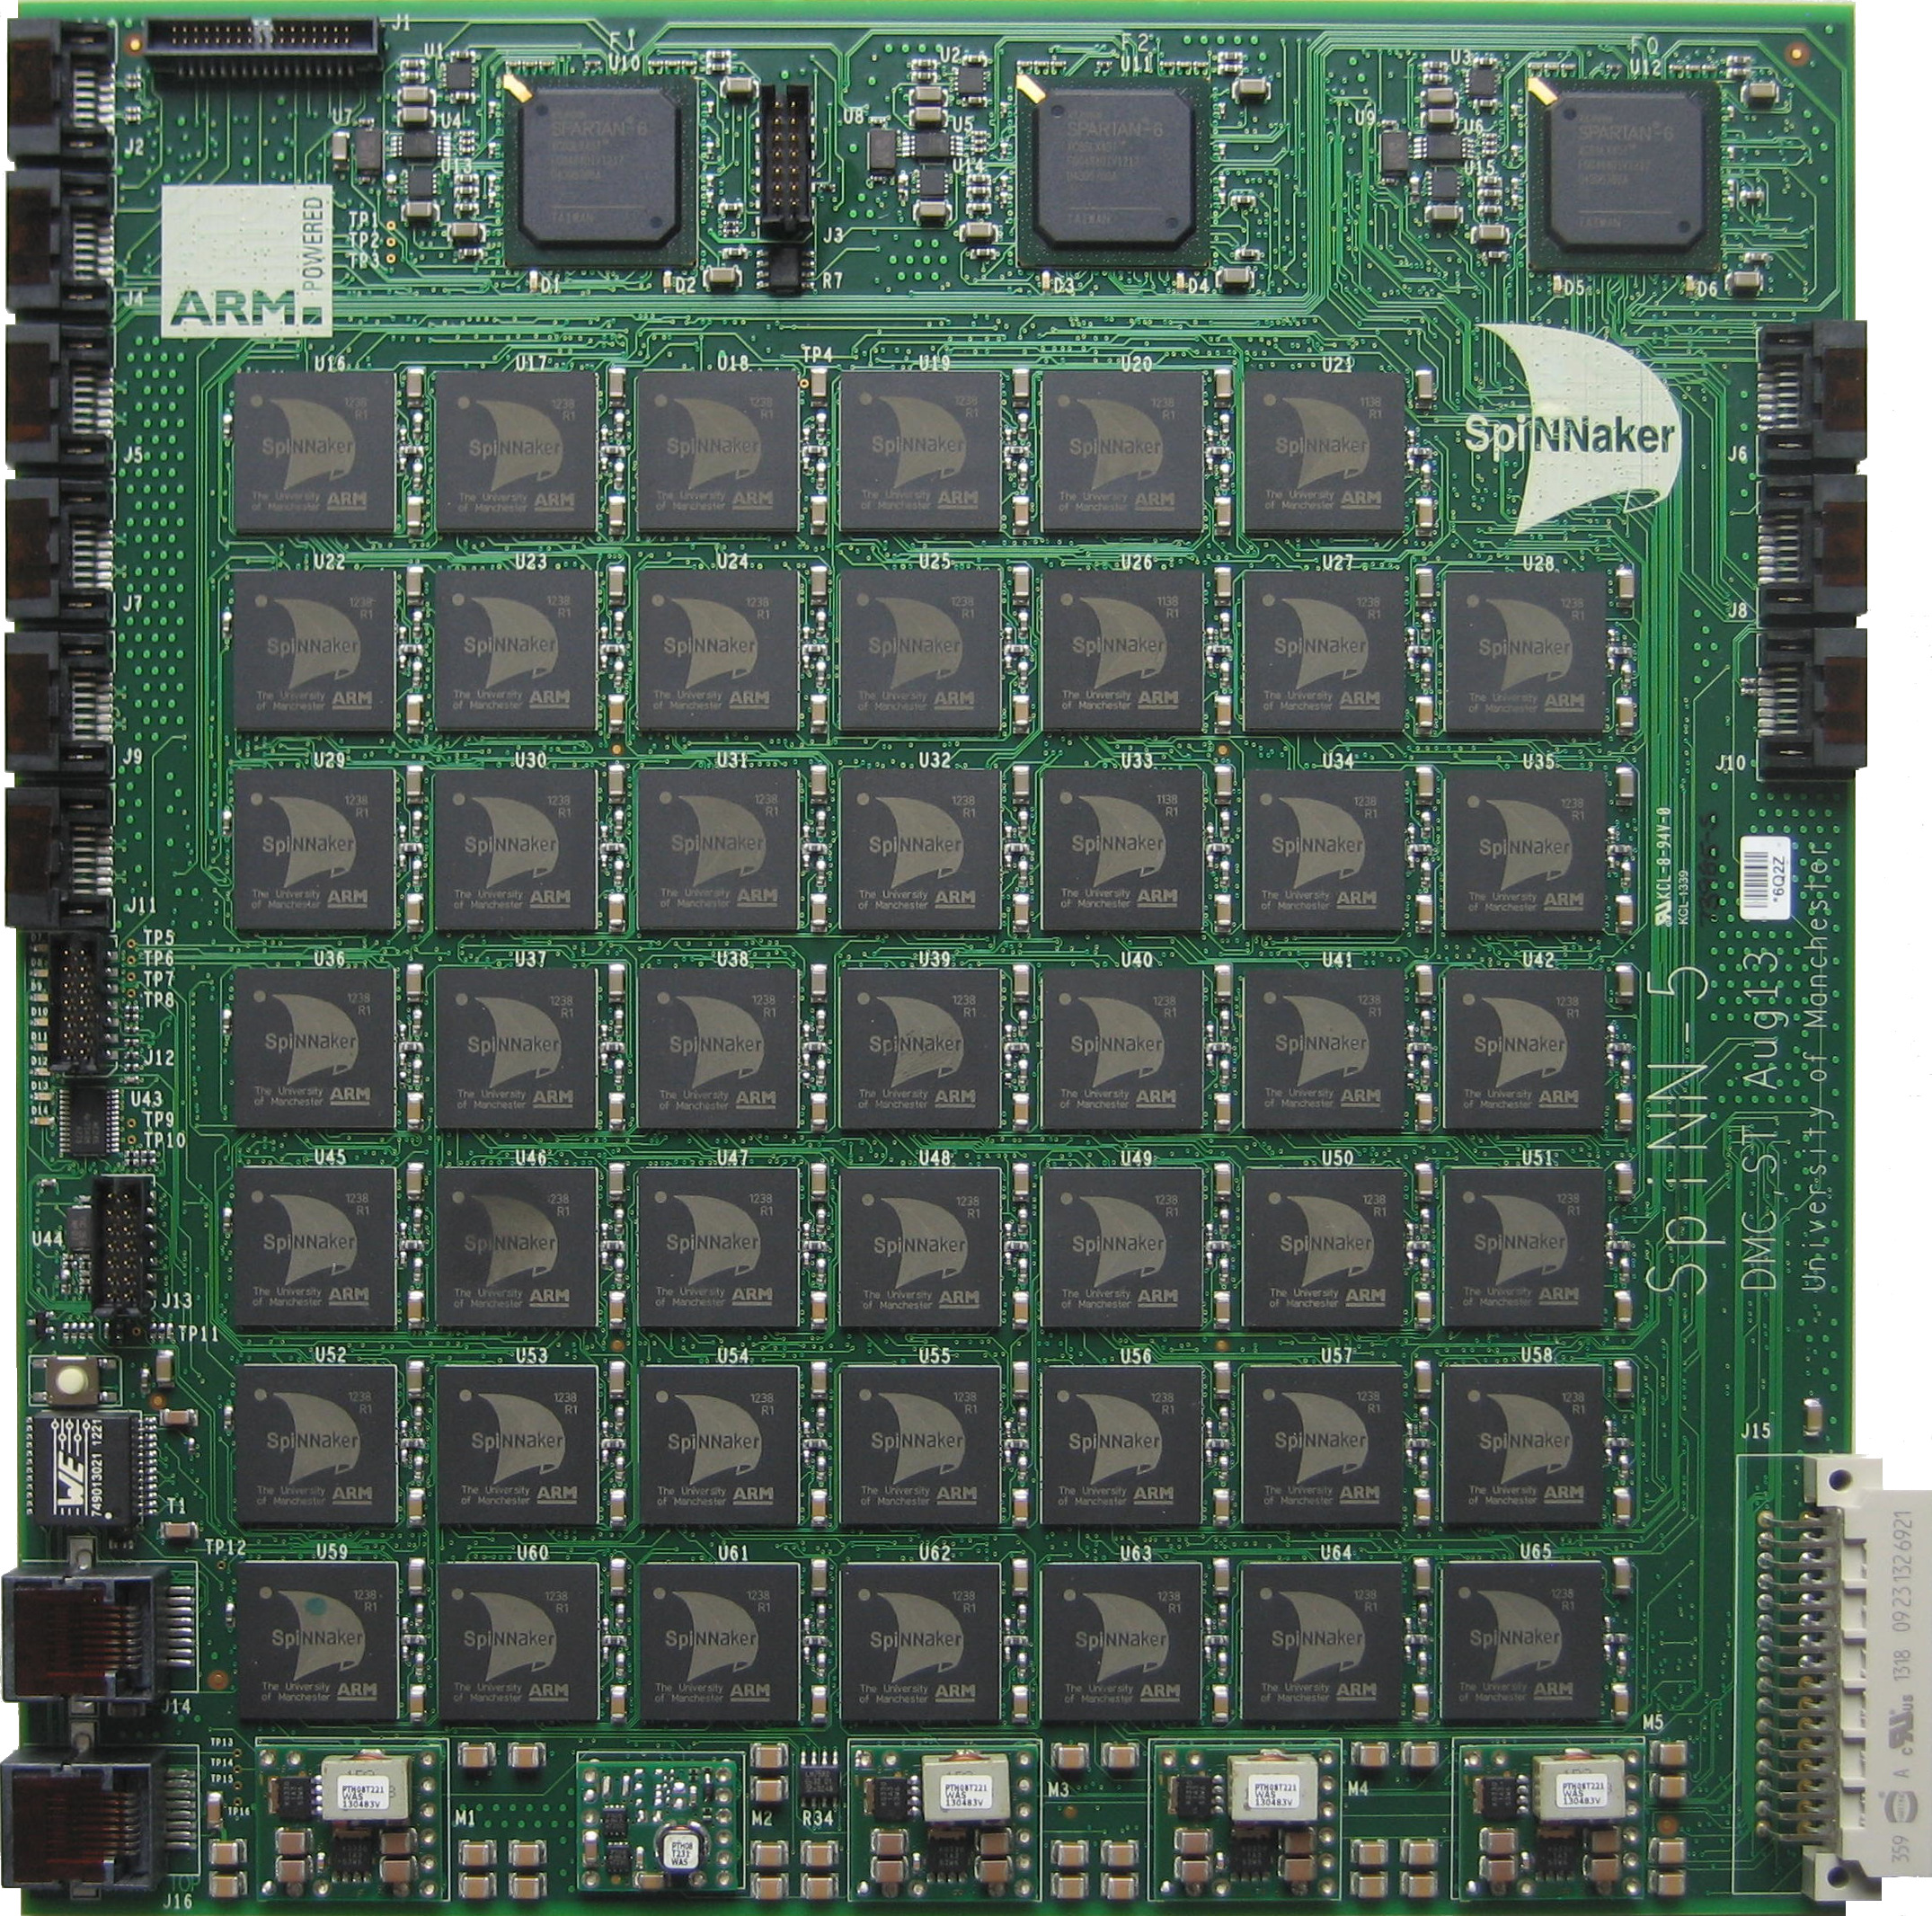
\includegraphics[width=\linewidth]{spinnakerBoard.jpg}
  \caption{A single SpiNNaker board with 48 SpiNNaker
    chips. Each chip has 18 cores.}
\end{figure}

\begin{figure}[H]
  \includegraphics[width=\linewidth]
    {SpiNNaker_9cabinets.jpg}
  \caption{The one million core machine in Manchester.
    It is capable of running up to one billion spiking
    neurons in real-time.}
\end{figure}

\end{appendices}

\end{document}
